\documentclass[main.tex]{subfiles}
\begin{document}

\chapter{Hamiltonian mechanics}
In this chapter, we'll study how a symplectic structure may be used to produce a dynamics on the manifold. This is accomplished by using so-called Hamiltonian vector fields. The physical interpretation of the whole construction will be given, and we'll conclude by proving a result about the general properties of the dynamical systems we get in this way.

\section{Hamiltonian vector fields}
\begin{definition}
	Given $h \in \Cinfty(M)$ on a symplectic manifold $(M, \omega)$, the \textbf{Hamiltonian vector field associated to $h$} is the vector field $X_h \in \fields(M)$ such that
	\begin{eqalign}
		\ipr{X_h} \omega = dh
	\end{eqalign}
	or equivalently\footnotemark
	\begin{eqalign}
		X_h = \omega^{-1}(dh).
	\end{eqalign}
\end{definition}
\footnotetext{Again, with $\omega^{-1}$ we mean the inverse of the isomorphism $\omega^\# : TM \isoto T^*M, X \mapsto \ipr{X}\omega$.}

\begin{definition}
	A vector field $X \in \fields(M)$ is \textbf{Hamiltonian} iff there exists a function $h \in \Cinfty(M)$ such that
	\begin{eqalign}
		\ipr{X} \omega = dh.
	\end{eqalign}
	The subset of Hamiltonian fields is denoted by $\hamfields(M)$.
\end{definition}

Notice \textbf{the Hamiltonian condition is equivalent to require $\ipr{X}\omega$ to be exact}. By analogy then we could conceive the following definition:

\begin{definition}
	A vector field $X \in \fields(M)$ is \textbf{symplectic} iff
	\begin{eqalign}
		d(\ipr{X}\omega) = 0.
	\end{eqalign}
	The subset of symplectic fields is denoted by $\sympfields(M)$.
\end{definition}

\begin{remark}
\label{rmk:symp_cohomology_is_dr_cohomology}
	These two kinds of fields are related in the same way exact and closed form are related:
	\begin{diagram}
	\label{diag:ham_symp_fields_inclusions}
		B^1(M) \arrow{d}{\omega^{-1}} \arrow[relation=\subseteq]{r} \&[-3ex] Z^1(M) \arrow{d}{\omega^{-1}} \arrow[relation=\subseteq]{r} \&[-3ex] \Omega^1(M) \arrow{d}{\omega^{-1}}\\
		\hamfields(M) \arrow[relation=\subseteq]{r} \& \sympfields(M) \arrow[relation=\subseteq]{r} \& \fields(M)
	\end{diagram}
	Moreover, $\omega^{-1}$ carries the $\R$-module structure downstairs: indeed, the linear combination of Hamiltonian (resp. symplectic) fields is still Hamiltonian (resp. symplectic). \textbf{This means the obstructions for a symplectic vector field to be an Hamiltonian one are encoded by the same cohomology data for differential forms}, i.e. the module $H^1_{dR}(M)$. If one wonders wheter this could be extended to a whole cohomology theory, the answer is \emph{yes}, although we'll need to wait the more general context of Poisson manifolds. The ``symplectic cohomology'' we'll get, however, will be canonically isomorphic to de Rham cohomology, as the first cohomology witnesses. As remarked in the previous chapter, this means that this flavor of cohomology is not enough to discern symplectic structures on $M$.
\end{remark}

\begin{remark}
\label{rmk:omega_is_const_on_symp_fields}
	An equivalent condition for a vector field to be symplectic can be obtained through Cartan's formula. In fact,
	\begin{eqalign}
		d\ipr{X}\omega = d\ipr{X}\omega + \cancel{\ipr{X}d\omega} = \Lie{X}\omega,
	\end{eqalign}
	so that a vector field is symplectic if and only if
	\begin{eqalign}
		\Lie{X} \omega = 0.
	\end{eqalign}
\end{remark}

\begin{example}
	Let $M = T^2$ with symplectic form $\omega = d\theta_1 \wedge d\theta_2$. The chosen coordinates represent angle variables around two closed circles around the torus, (for simplicity, we can think of them to be around the ``principal'' directions of the torus). Consider the fields $X_1 = \partial_{\theta_1}$ and $X_2 = -\partial_{\theta_2}$: they are symplectic but not Hamiltonian. Indeed, $\Lie{X_i} \omega = 0$ for both $i=1,2$ but
	\begin{eqalign}
		\ipr{X_1} \omega = d\theta_{2}
		\qquad \text{and} \qquad
		\ipr{X_2} \omega = d\theta_{1}
	\end{eqalign}
	which is \textbf{not} exact since $\theta_i$ can't be defined globally\footnote{Variables $\theta_1$ and $\theta_2$ are multivalued on $T^2 = \R^2/(2\pi\Z)^2$, for instance $(0,\theta_2) = (2\pi, \theta_2)$. We cannot restrict these coordinates to $[0, 2\pi)$ to define a cohomology otherwise they would be discontinuous, for instance $\theta_1$ would have a discontinuity at $(0, \theta_2)$.}: they are only defined locally (at most on the whole torus with two independent\footnote{Non-homotopic, non-contractible loops which wind once.} circles removed). Anyway, $d\theta_i$ does define a differential $1$-form on the whole space (intuitively, since differentiating eliminates the $2\pi$ jump discontinuity which prevents a global definition). Actually this is the whole point of the first cohomology group: $\overline{d\theta_1}, \overline{d\theta_2}$ generate $H^1_{dR}(T^2)$ which is, indeed, $\R \times \R$:
	\begin{eqalign}
		H^1_{dR}(T^2) = \langle \overline{d\theta_1}, \overline{d\theta_2} \rangle \iso \R \times \R .
	\end{eqalign}
\end{example}

\begin{theorem}
\label{th:flow_of_symp_field}
	The $1$-parameter group of diffeomorphisms $\phi_t : M \isoto M$ associated to a symplectic vector field $X$ preserves the symplectic structure:
	\begin{eqalign}
	\label{eq:ham_flow_sympl}
		\phi_t^* \omega = \omega.
	\end{eqalign}
	This means that \textbf{the group is actually a group of symplectomorphisms}.
\end{theorem}
\begin{proof}
	Follows from Equation~\ref{eq:t_depend_Lie_derivative} and Remark~\ref{rmk:omega_is_const_on_symp_fields}. Indeed let $\phi_t : M \to M$ be associated to $X_h = \omega^{-1}(dh)$. Then 
	\begin{eqalign}
		\der{}{t}(\phi_t^*(\omega))=\phi_t^* \Lie{X_h}\omega = \phi_t^* (d\ipr{X_h}\omega + \ipr{X}\cancel{d\omega}) = \phi_t^*(\cancel{d^2 h}) = 0 .
	\end{eqalign}
\end{proof}

\begin{example}
\label{ex:sphere_with_height_ham}
	Let $M=S^2$ with the symplectic structure given by the mixed product introduced in Example~\ref{ex:eu_sp_sphere}. Consider the immersion given by cylindrical coordinates
	\begin{eqalign}
		\iota : S^2 &\longto \R^3\\
		(\theta,h) &\longmapsto (\sqrt{1-h^2} \cos \theta,\, \sqrt{1-h^2}\sin \theta,\, h).
	\end{eqalign}
	Then $T\iota(S^2)$ is described by
	\begin{eqalign}
		\iota_*(\partial_\theta) &= \pder{x}{\theta} \pder{}{x} + \pder{y}{\theta} \pder{}{y} + \pder{z}{\theta} \pder{}{z} = -y \partial_x + x\partial_y\\[2ex]
		\iota_*(\partial_h) &= \pder{x}{h} \pder{}{x} + \pder{y}{h} \pder{}{y} + \pder{z}{h} \pder{}{z} = - \frac{xz}{1-z^2}\partial_x - \frac{yz}{1-z^2}\partial_y + \partial_z
	\end{eqalign}
	where in the second computation we made the substitution $\cos \theta = x/\sqrt{1-z^2}$ and $\sin \theta = y/\sqrt{1-z^2}$. We use these to compute the symplectic form in coordinates. In truth, we already know
	\begin{eqalign}
		\omega(\partial_\theta, \partial_\theta) = \omega(\partial_h, \partial_h) = 0
	\end{eqalign}
	by antisimmetry, so we just go for the mixed one:
	\begin{eqalign}
		\omega(\partial_\theta, \partial_h)(x, y, z) &= \langle (x,y,z), \iota_* (\partial_\theta) \times \iota_*(\partial_h) \rangle\\
		&= \langle (x,y,z), \frac{y^2z}{1-z^2}\partial_z + y \partial_y + \frac{x^2z}{1-z^2}\partial_z + x\partial_x \rangle\\
		&= \langle (x,y,z), x \partial_x + y \partial_y + \frac{\cancelto{1}{(x^2+y^2)} z}{\cancelto{1}{1-z^2}} \partial_z \rangle\\
		&= 1.
	\end{eqalign}
	So that $\omega = d\theta \wedge dh$.

	Now consider $h \in \Cinfty(M)$ given by the ``height function'', so --- by an happy coincidence of notations --- literally the coordinate $h$ on $S^2$. Its Hamiltonian field is defined by $\ipr{X_h}\omega = dh$ so that $X_h = \partial_\theta$, whose $1$-parameter group of diffeomorphisms is $\phi_t(\theta, h) = (\theta + t, h)$ (a rotation of angle $t$), which evidently preserves the form $\omega$.
\end{example}

\begin{theorem}
	Let $h \in \Cinfty(M)$. Then $h$ is constant along the flow of $X_h$.
\end{theorem}
\begin{proof}
	We check $X_h(h)$, the derivative of $h$ along the field $X_h$:
	\begin{eqalign}
		\Lie{X_h}h = X_h(h) = dh(X_h) = \ipr{X_h} dh = \ipr{X_h} \ipr{X_h} \omega = 0.
	\end{eqalign}
\end{proof}
\begin{corollary}
	Integral curves of $X_h$ are contained in the level sets of $h$.
\end{corollary}

Indeed, in Example~\ref{ex:sphere_with_height_ham} we took the height function on the sphere as Hamiltonian an indeed the group we got was rotations at a fixed height, i.e. the flow lines were parallels on the sphere.

\section{Physical meaning of a symplectic structure}
We'd like now to justify our mathematical definitions in terms of the properties we want an Hamiltonian physical model to have.

\begin{construction}
\label{const:symp_struct_for_ham_mechanics}
	The starting point of any such model is the space of possible physical states of a chosen physical system, i.e. the set of its \emph{positions} and its \emph{momenta}. This is assumed to form a smooth manifold $M$, called the \emph{phase space}. \textbf{We model physics as some rule associating, to a given energy function $h \in \Cinfty(M)$, an evolution of the physical state on the phase space}. We can think of such an evolution as the flow of a vector field $X_h$ associated to $h$, although it should only depend on energy \emph{differences} between states, hence on $dh$.

	To produce such a vector field we necessarily need to make a choice of equations: this is where physical experience enters in the model. In the simplest case, we adopt Newton equations:
	\begin{eqalign}
		F = - \der{U}{x} = m \ddot{x}
	\end{eqalign}
	which can be rewritten in terms of
	\begin{eqalign}
		h = \frac{(m \dot x)^2}{2m} + U(x) = \underbrace{K(\dot x)}_{\text{kinetic energy}} + \underbrace{U(x)}_{\text{potential energy}}
	\end{eqalign}
	as
	\begin{eqalign}
		\begin{dcases}
			\dot x = \frac1m \bigpder{h}{\dot x}\\
			\ddot x = - \frac1m \bigpder{h}{x}
		\end{dcases}
	\end{eqalign}
	i.e. in matrix representation
	\begin{eqalign}
		\der{}{t} \begin{pmatrix} x \\ m\dot x \end{pmatrix} = \begin{pmatrix} 0 & 1\\-1 & 0\end{pmatrix}\underbrace{\begin{pmatrix}\partial_x h \\ \partial_{m\dot x} h\end{pmatrix}}_{dh}
	\end{eqalign}
	The dependence of $X_h$ on $dh$ is then \emph{linear}, meaning it can be given at each point $p \in M$ by a linear map $\eta^\# : T^*_pM \to T_pM$, so that $X_h = \eta^\# (dh)$. Geometrically, such a smooth choice of linear maps is encoded by the tensor field $\eta \in \Gamma(TM \tens TM)$ associated to $\eta^\#$. In this sense, \textbf{$\eta$ is the mathematical incarnation of the laws of physics, because it associates evolution to energy}. If we \emph{assume}\footnote{This is not always true! We'll see some instances of this and we'll introduce a formalism to treat those cases as well, the one of \emph{Poisson manifolds}.} all energy gradients produce a non-zero dynamics then $\eta$ is non-degenerate\footnote{Which is equivalent to assume the injectivity of $\eta^\#$. In this case we can define $(\eta^\#)^{-1} =: \omega^\# : TM \to T^*M$ and its associated tensor $\omega \in \Gamma(T^*M \tens T^*M)$.}; hence we can work with its ``inverse'' (pointwise as a map) instead, call it $\omega \in \Gamma(T^*M \tens T^*M)$.

	Now properties of $\omega$, which is our ``wannabe'' symplectic form, will come from two additional modelling assumption. \textbf{The first is conservation of energy}, which is the condition $X_h(h) = 0$. Expressed in terms of $\omega$, it becomes\footnote{We can rewrite $X_h(h) = \langle X_h, dh \rangle = \langle X_h, \omega^\#(\eta^\#(dh)) \rangle = \langle X_h, \omega^\#(X_h) \rangle = \omega(X_h, X_h)$.} $\omega(X_h, X_h) = 0$. Since this has to be satisfied by \emph{all} choices $h \in \Cinfty(M)$, including --- locally --- the coordinate functions $x^i$ (thus on a local frame for $TM$), hence, locally, $\omega(X,X) = 0$ for any vector field $X$, which means $\omega$ is skew-symmetric ($\omega \in \Omega^2(M)$).

	\textbf{The second assumption is that laws of physics are time-independent}, which translates mathematically to:
	\begin{eqalign}
		\phi_t^*\omega = \omega
	\end{eqalign}
	where $\phi_t : M \to M$ is the flow of $X_h$. Notice, again, this must be true for any choice of $h$, so that by the same computation we did to prove Theorem~\ref{th:flow_of_symp_field}, it implies\footnote{The condition $\phi_t^*\omega = \omega$ is equivalent to $0 = \Lie{X_h}\omega = (d\ipr{X_h} + \ipr{X_h}d)\omega = d(\ipr{X_h}\omega)+\ipr{X_h}d\omega = \cancel{d^2h} + \ipr{X_h}d\omega$. Since this has to hold for any choice of $h$ it implies $d\omega=0$.} $d\omega = 0$.
\end{construction}

Now let $M=T^*X$ for some smooth manifold $X$, which we think as to represent the configuration space of a mechanical system, and let $\omega = -d\alpha = dx^j \wedge d\xi_j$ be the canonical symplectic structure on $M$. Fix a function $h \in \Cinfty(T^*X)$. Then its Hamiltonian vector field is obtained by applying the graded Leibniz rule for the interior product\footnotemark:
\begin{eqalign}
	X_h = \pder{h}{\xi_j} \partial_{x^j} - \pder{h}{x^j}\partial_{\xi_j}
\end{eqalign}
\textbf{which corresponds very naturally to the vector field we got from Newton's equations}. Indeed, they're the same up to rescaling by a factor $1/m$. Somehow, this ``trick'' to lower Newton's equations to the first-order, when taken seriously and globally on the configuration space, gives us the symplectic structure of $T^* X$.
\footnotetext{Explicitly:
\begin{eqalign}
	\ipr{X_h}\omega &= (dx^j \wedge d\xi_j) \left(\pder{h}{\xi_i} \partial_{x^i} - \pder{h}{x^i}\partial_{\xi_i}, -\right) = dx^j\left(\pder{h}{\xi_i} \partial_{x^i}\right) d\xi_j - d\xi_j\left(- \pder{h}{x^i}\partial_{\xi_i}\right)dx^j\\
	& = \pder{h}{x^j}dx^j + \pder{h}{\xi_j} d\xi_j = dh.
\end{eqalign}}

\section{Poisson brackets}
We've seen in the previous sections that the dynamics on a symplectic manifold comes, in the first place, from a function $h \in \Cinfty(M)$. Moreover, in the physical interpretation of a symplectic manifold we can also imagine the smooth functions on $M$ to represent observables of the system, i.e. quantities we can measure at any given state $p \in M$. Then we might try to find a way to study not only the dynamics of the system, but also the dynamics of the observables themselves.

To do this, we introduce a formalism which relies solely on the functions $\Cinfty(M)$. It will be so powerful that, as we'll see later in these notes, we will able to dispense with the fields $X_h$ altogether.

\begin{definition}
	The \textbf{Poisson brackets} of two functions $f,g \in \Cinfty(M)$ is defined as
	\begin{eqalign}
		\{ f, g \} = \omega(X_f, X_g).
	\end{eqalign}
\end{definition}

Notice $\omega(X_f, X_g) = (\ipr{X_f}\omega)(X_g) = \langle df, X_g \rangle = X_g (f)$, hence $\{ f, g \} = X_g(f) = - X_f(g)$.

\begin{definition}
	A \textbf{Poisson algebra} $(\mathcal P, \{-,-\})$ is a commutative associative algebra $\mathcal P$ equipped with an additional Lie algebra structure $\{-,-\}$ which satisfy a Leibniz rule relative to the algebra product:
	\begin{eqalign}
		\{f, gh\} = \{f,g\}h + g\{f,h\}, \quad \forall f,g,h \in \mathcal P.
	\end{eqalign}
\end{definition}

\begin{theorem}
	For all $f,g,h \in \Cinfty(M)$, the Poisson brackets satisfy the following properties:
	\begin{enumerate}
		\item \textbf{Bilinearity}:
		\begin{eqalign}
			\{ \alpha f + \beta g, h\} = \alpha \{ f, g \} + \beta \{g,h\}
		\end{eqalign}
		for any $\alpha, \beta \in \R$;
		\item \textbf{Skew-symmetry}:
		\begin{eqalign}
			\{ f,g\} = -\{g,f\};
		\end{eqalign}
		\item \textbf{Leibniz rule}:
		\begin{eqalign}
			\{ f, gh \} = \{f,g\}h + g\{f,h\}
		\end{eqalign}
		for all $f,g,h \in \Cinfty(M)$;
		\item \textbf{Jacobi identity}:
		\begin{eqalign}
			\{f, \{g,h\}\} + \{g, \{h, f\}\} + \{h, \{ f,g\} \} = 0
		\end{eqalign}
		for all $f,g,h \in \Cinfty(M)$.
	\end{enumerate}
\end{theorem}
\begin{proof}
Direct computation.
\end{proof}

\begin{corollary}
	The Poisson brackets puts a Poisson algebra structure on $\Cinfty(M)$, i.e. $(\Cinfty(M), \{ - , -\})$ is a Poisson algebra
\end{corollary}

\begin{theorem}
\label{th:comm_is_ham}
	Let $U, V \in \sympfields(M)$ be symplectic vector fields, then
	\begin{eqalign}
		[U, V] = -X_{\omega(U,V)}
	\end{eqalign}
\end{theorem}
\begin{proof}
	Fix an atlas, we'll verify $\ipr{[U,V]} \omega = -d(\omega(U,V))$ using coordinates computation. We'll use of the following facts (the order reflects where they are used in the computation):
	\begin{enumerate}
		\item The Lie derivative of a tensor is found by successively saturating the involved indices\footnotemark (one for the derivative + all the indices of the tensor) with the vector field we are differentiating along, so in particular for a $1$-form, it is
		\begin{eqalign}
			\Lie{U} \eta = \left[ U^\mu (\partial_\mu \eta_\beta) + (\partial_\beta U^\mu) \eta_\mu \right] dx^\beta;
		\end{eqalign}
		while for a $2$-form, it is
		\begin{eqalign}
			\Lie{U} \omega = \left[ U^\mu (\partial_\mu \omega_{\alpha\beta})  + (\partial_\alpha U^\mu) \omega_{\mu\beta} + (\partial_\beta U^\mu) \omega_{\alpha \mu} \right] dx^\alpha \wedge dx^\beta.
		\end{eqalign}
		\item Cartan's Magic Formula \eqref{eq:cartan_magic_formula}.
		\item The fields $U$ and $V$ are symplectic, hence
		\begin{eqalign}
			d\ipr{U}\omega = d\ipr{V}\omega = 0.
		\end{eqalign}
	\end{enumerate}
	\footnotetext{The Lie derivative of a $k$-form $\omega$ is given by the extension of the Leibniz rule
	\begin{eqalign}
		\Lie{U}(\langle \omega, \partial_{\alpha_1}, \dots, \partial_{\alpha_k} \rangle) = \langle \Lie{U}\omega, \partial_{\alpha_1}, \dots, \partial_{\alpha_k} \rangle + \langle \omega, \Lie{U}\partial_{\alpha_1}, \dots, \partial_{\alpha_k} \rangle + \dots + \langle \omega, \partial_{\alpha_1}, \dots, \Lie{U}\partial_{\alpha_k} \rangle
	\end{eqalign}
	i.e.
	\begin{eqalign}
		(\Lie{U}\omega)(\partial_{\alpha_1}, \dots, \partial_{\alpha_k}) & = U^\mu \partial_\mu ( \omega ( \partial_{\alpha_1}, \dots, \partial_{\alpha_k} )) - \omega([U, \partial_{\alpha_1}], \dots \partial_{\alpha_k}) - \dots - \omega(\partial_{\alpha_1}, \dots , [U, \partial_{\alpha_k}]) \\
		& = U^\mu \partial_\mu ( \omega ( \partial_{\alpha_1}, \dots, \partial_{\alpha_k} )) + (\partial_{\alpha_1} U^{\alpha_1})\omega(\partial_{\alpha_1}, \dots \partial_{\alpha_k}) + \dots + (\partial_{\alpha_k} U^{\alpha_k})\omega(\partial_{\alpha_1}, \dots , \partial_{\alpha_k}) 
	\end{eqalign}
	}

	Together with the above facts, two algebraic tricks are used:

	\begin{enumerate}
		\item In the second line, we use the ``inverse'' Leibniz rule:
		\begin{eqalign}
			(\partial_\mu V^\alpha) \omega_{\alpha\beta} = \partial_\mu (V^\alpha \omega_\alpha \beta) - V^\alpha (\partial_\mu \omega_{\alpha\beta})
		\end{eqalign}
		\item In the third line, we add and substract the identical terms marked in blue.
	\end{enumerate}

	The computation goes like this:

	\begin{equation}
		\begin{aligned}
			\ipr{[U,V]} \omega &= \left( U^\mu (\partial_\mu V^\alpha) - V^\mu (\partial_\mu U^\alpha) \right) \omega_{\alpha\beta} dx^\beta\\
			&= U^\mu \partial_\mu (V^\alpha \omega_{\alpha\beta}) dx^\beta - U^\mu V^\alpha (\partial_\mu \omega_{\alpha\beta}) dx^\beta - V^\mu (\partial_\mu U^\alpha) \omega_{\alpha\beta}dx^\beta\\
			&= U^\mu (\partial_\mu V^\alpha \omega_{\alpha\beta}) dx^\beta \textcolor{blue}{+ (\partial_\beta U^\mu) V^\alpha \omega_{\alpha \mu} dx^\beta}\\
			&\quad - U^\mu V^\alpha (\partial_\mu \omega_{\alpha\beta}) dx^\beta - V^\alpha (\partial_\alpha U^\mu) \omega_{\mu\beta}dx^\beta \textcolor{blue}{- V^\alpha (\partial_\beta U^\mu) \omega_{\alpha \mu} dx^\beta}\\
			&= \Lie{U} (\ipr{V} \omega) - \ipr{V} (\Lie{U}\omega)\\
			&= d \ipr{U} \ipr{V} \omega - \ipr{U} \cancel{d\ipr{V} \omega} - \ipr{V} \cancel{d \ipr{U} \omega} + \cancel{\ipr{V} \ipr{U} d\omega}\\
			&= -d (\omega(U,V)).
		\end{aligned}
	\end{equation}
	Then the theorem is proved by definition of Hamiltonian vector.
\end{proof}

\begin{remark}
	A fruitful reading of the last theorem is \textbf{the set of symplectic fields is closed under the operation of taking commutators}. The same applies to Hamiltonian fields since the result of the commutators is Hamiltonian and Hamiltonian vectors are symplectic. Therefore, the downstairs inclusions of Diagram~\ref{diag:ham_symp_fields_inclusions} get promoted to inclusions of Lie algebras:
	\begin{eqalign}
		\hamfields(M)\ \underset{\cat{LieAlg}}\subseteq\ \sympfields(M)\ \underset{\cat{LieAlg}}\subseteq\ \fields(M).
	\end{eqalign}
\end{remark}

\begin{corollary}
	The Poisson bracket puts a Lie algebra structure on $\Cinfty(M)$, and the assignment of the Hamiltonian field
	\begin{eqalign}
		(\Cinfty(M), \{-,-\}) &\longto (\fields^{\text{Ham}}(M), [-,-])\\
		f &\longmapsto X_f
	\end{eqalign}
	is an \textbf{anti}morphism of Lie algebras, since
	\begin{eqalign}
		X_{\{f,g\}} = - [X_f, X_g]
	\end{eqalign}
	Such morphism is surjective (by the very definition of Hamiltonian vector field), but not injective (as $f$ and $f+\cost$ have clearly the same image under this map).
\end{corollary}

The flow $\phi_t$ of $X_h$ encodes the evolution of the state of the system under the Hamiltonian function $h \in \Cinfty(M)$. Evaluating $f$ on $\phi_t$ makes $f$ a function of time, thus providing a function $f(t)$ which spits out the value of $f$ on the state reached by the system at $t$. Using the Poisson brackets, we can skip a step and get the evolution of $f$ directly:

\begin{theorem}
	Let $f, h \in \Cinfty(M)$. Then the evolution of $f$ on the flow of $X_h$ is given by the bracket with $h$:
	\begin{eqalign}
		\der{f}{t} = \{f, h\}
	\end{eqalign}
\end{theorem}
\begin{proof}
	\begin{eqalign}
		\der{f}{t} = X_h(f) = \langle X_h, \ipr{X_f}\omega \rangle = \ipr{X_h}\ipr{X_f}\omega = \omega(X_f, X_h) = \{f,h\}.
	\end{eqalign}
\end{proof}

\section{Integrable systems}
\begin{definition}
	We call \textbf{Hamiltonian system} the data of a symplectic manifold together with a fixed choice of Hamiltonian $h \in \Cinfty(M)$.
\end{definition}

\begin{definition}
	Let $(M, \omega, h)$ be an Hamiltonian system. A function $f \in \Cinfty(M)$ such that $\{f,h\} = 0$ is called an \textbf{integral of motion} of the system.
\end{definition}

The great insight of Hamiltonian formalism is that \textbf{integrals of motion are the key to describe explicitly the evolution of a system.} This intuition can be justified by the geometrical treatment we have given so far. Hence this section will be devoted to this purpose, and will culminate with a structural result about Hamiltonian systems, the Arnold--Liouville Theorem.

\begin{definition}
	A set of functions $f_1, \ldots, f_k \in \Cinfty(M)$ is said to be \textbf{in involution} or to \textbf{commute} if
	\begin{eqalign}
		\{f_i, f_j \} = 0, \quad \forall i,j \leq k.
	\end{eqalign}
\end{definition}

\begin{construction}
\label{const:level_submanifolds_of_involutions}
	Let $(M, \omega)$ be a $2n$-dimensional symplectic manifold, let $h_1, \ldots, h_n$ be functions in involution and let finally $c \in \R^n$ be a regular value of
	\begin{eqalign}
		H : M &\longto \R^n\\
		p &\longmapsto (h_1(p), \ldots, h_n(p))
	\end{eqalign}
	meaning that $dh_1\vert_p, \ldots dh_n \vert_p$ are linearly independent at each $p \in H^{-1}(c)$.

	By the implicit function theorem, \textbf{$H^{-1}(c)$ is a submanifold of $M$ and its tangent spaces are generated by the Hamiltonian vector fields associated to the functions $h_1, \ldots, h_n$}: indeed,
	\begin{eqalign}
		T_pH^{-1}(c) = \{ X_p \in T_pM \suchthat X_p(h_i)=0\ \forall i \leq n \}
	\end{eqalign}
	and
	\begin{eqalign}
		X_{h_i}(h_j) = \omega(X_{h_i}, X_{h_j}) = \{ h_i, h_j \} = 0
	\end{eqalign}
	and the $X_{h_i}$ are independent. Moreover, \textbf{this computation also shows $H^{-1}(c)$ is a Lagrangian submanifold of $M$}, since it has dimension $n$ and $\omega$ vanishes on its generators. Then $H$ is said to be a \textbf{Lagrangian fibration}.
\end{construction}

\begin{definition}
	A set of functions $f_1, \ldots, f_k \in \Cinfty(M)$ is said to be \textbf{independent} if
	\begin{eqalign}
		\text{$\forall p \in M, df_1\vert_p, \ldots, df_n\vert_p$ are linearly independent over $T^*M$.}
	\end{eqalign}
\end{definition}

Construction~\ref{const:level_submanifolds_of_involutions} then shows that:

\begin{lemma}
\label{lemma:isotropic_dist}
	A set $f_1, \ldots, f_k$ of functions independent and in involution generates an \textbf{isotropic distribution}, which means at every point $x \in M$ they span a subspace of $T_xM$ depending smoothly on $x$
	\begin{eqalign}
		\langle X_{f_1}\vert_x, \ldots, X_{f_k}\vert_x \rangle \underset{\cat{Vec}}\subseteq T_x M
	\end{eqalign}
	such that
	\begin{eqalign}
		\omega(X, Y) = 0, \quad \forall X,Y \in \langle X_{f_1}, \ldots, X_{f_k} \rangle.
	\end{eqalign}
	In particular, when $k = \frac12 \dim M$, the distribution is Lagrangian.
\end{lemma}

\begin{definition}
	An Hamiltonian system $(M, \omega, h)$ is called \textbf{completely integrable} if it possesses $n=\frac12 \dim M$ integrals of motion which are independent and in involution.
\end{definition}

\section{Arnold--Liouville Theorem}
\begin{example}[Pendulum]
\label{ex:pendulum}
	When $\dim M=2$, every Hamiltonian system whose energy function $h$ is not closed ($dh \neq 0$) is an integrable system (because we need just one function, and we have $h$ already). The configuration space of a simple pendulum is $S^1$, and thus $M = T^*S^1 \iso S^1 \times \R$ is such a $2$-dimensional Hamiltonian system, with Hamiltonian given by the energy function:
	\begin{eqalign}
		h(\theta, \xi) = \frac{\xi^2}{2m \ell^2} +m\ell (1-\cos \theta)
	\end{eqalign}
	where $m$ is the mass of the pendulum and $\ell$ the length of the rod. The parameter $\theta$ will refer to the anticlockwise angle measured from the down direction. We choose units as to have $m=\ell=1$. Then
	\begin{eqalign}
		h(\theta, \xi) = \frac{\xi^2}2 + 1-\cos \theta.
	\end{eqalign}

	We plot the level sets of $h$:

	\begin{figure}[H]
		\centering
		\begin{tikzpicture}
			\node (image) at (0,0) {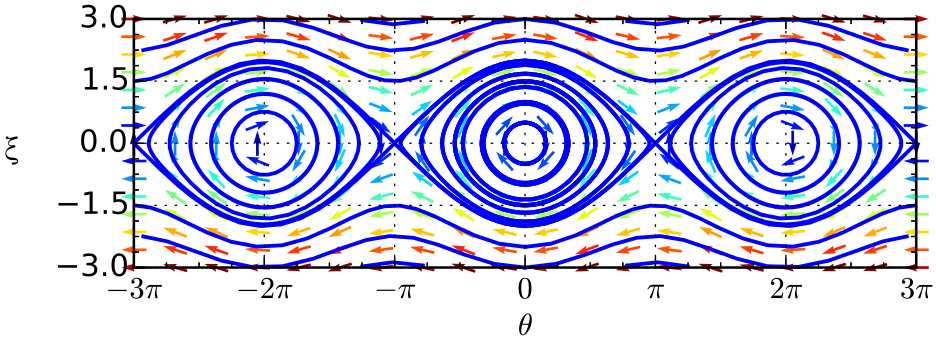
\includegraphics[width=.85\textwidth]{figures/pendulum_phase_space.png}};
		\end{tikzpicture}
		\caption{}
		\label{fig:pendulum_phase_diagram}
	\end{figure}

	The critical points of $h$ can be read from the expression of $dh$: $\xi d\xi + \sin \theta d\theta$, and are
	\begin{eqalign}
		\xi = 0, \quad \theta = 0,\, \pm \pi
	\end{eqalign}
	In these points, the system is not integrable anymore (as $h$ is not regular, see Construction~\ref{const:level_submanifolds_of_involutions}), so we remove them from the manifold $M$. In this new manifold, which is again symplectic and smooth, the system is everywhere integrable and its integral submanifolds are either circles (for closed orbits) or copies of $\R$ (for the extremal orbit which is a circle with two points removed, as well as for larger orbits which are unaffected).
\end{example}

It is somewhat surprising that the fibration phenomenon we have seen at the end of Example~\ref{ex:pendulum} is not peculiar to that example: \textbf{integral submanifolds happen to be always tori or Euclidean spaces}. This is the subject of Arnold--Liouville Theorem.

We start with some vocabulary:

\begin{definition}
	A \textbf{locally trivial surjective submersion} is a surjective submersion $f: M \to N$ such that there exists a manifold $F$ and for every point $p \in N$ there exist an open neighbourhood $U$ and a diffeomorphism $f^{-1}(U) \isoto U \times F$ which makes the following commute:
	\begin{diagram}
		M \arrow[relation=\supset]{r} \&[-3ex] f^{-1}(U) \arrow[swap]{dr}{f} \arrow{rr}{\phi} \& \& U \times F \arrow{dl}{\pr_2}\\
		\& \& U
	\end{diagram}
\end{definition}

\begin{definition}
	A \textbf{proper map} $f: X \to Y$, where $X$ and $Y$ are topological spaces, is a continuous map such that $f^{-1}$ maps compact sets to compact sets.
\end{definition}

\begin{lemma}[{\cite{mo2019properness}}]
\label{lemma:subm_is_proper}
	Any surjective submersion with compact and connected fibers is proper.
\end{lemma}

\begin{lemma}[Ehresmann]
\label{lemma:ehresmann}
	Any proper surjective submersion is locally trivial.
\end{lemma}

\begin{theorem}[Arnold--Liouville]
\label{th:arnold_liouville}
	Let $(M, \omega)$ be a symplectic manifold equipped with $h_1, \ldots, h_n \in \Cinfty(M)$ functions in involution and define $H = (h_1, \ldots, h_n): M \to \R^n$. Suppose $H$ is a \textbf{Lagrangian fibration}; i.e. its fibers are Lagrangian submanifolds of constant dimension. Let $p \in M$ such that the flows of $X_{h_1}, \ldots, X_{h_n}$, starting at $p$, are complete\footnotemark, and call $F^{(p)}$ the connected component of $H^{-1}(H(p))$ containing $p$. Then
	\begin{enumerate}
		\item $F^{(p)}$ is diffeomorphic to $\R^{n-k} \times \T^k$ through a diffeomorphism that maps the flows of $X_{h_1}, \ldots, X_{h_n}$ to linear flows on $\R^{n-k} \times \T^k$; i.e. a linear $\R^n$-action on $\R^{n-k} \times \T^k$;
		\item in a neighbourhood of $F^{(p)}$ the functions $h_1, \ldots, h_n$ can be completed to a system of Darboux coordinates;
		\item the set $M_C$ of points whose fiber is compact is open, and $H\vert_{M_C}$ is a locally trivial Lagrangian fibration with fiber $\T^n$;
		\item in a neighbourhood of each fiber of $H\vert_{M_C}$ there exists a system of Darboux coordinates formed by $n$ angle variables on $\T^n$ and $n$ integrals of motion called \textbf{action variables} (where the term \emph{action} comes from their physical meaning).
	\end{enumerate}
	\footnotetext{Which means that the flow $\phi_t$ is defined for all $t \in \R$, or --- equivalently --- that it is infinitely prolongable. This is always the case when $M$ is compact.}
\end{theorem}
\begin{remark}
	The statement of \textbf{the theorem is agnostic about the choice of Hamiltonian function}. Indeed, it is not about Hamiltonian manifolds but about symplectic ones with $n$ functions in involution. Basically, this comes from the fact that the choice of $h$ is (from the mathematical point of view) arbitrary, since it comes from the physical situation: the mathematical content of the Hamiltonian formalism is given solely by the set of functions in involution.
\end{remark}
\begin{remark}
	The condition on $H$ is artificial since, following Example~\ref{ex:pendulum}, we can always remove from $M$ the critical points of $H$ and apply the theorem to $M\setminus \operatorname{crit}H$ (such a subset is always open, because it is the preimage of the open set of non-critical values). On this manifold $H$ is a fibration and by Construction~\ref{const:level_submanifolds_of_involutions} its fibers are Lagrangian.
\end{remark}
\begin{remark}
	To state the theorem globally (since any local statement about a symplectic manifold is trivial) we must ask for completeness of the flow. Indeed, to get fibers diffeomorphic to $\R$ and $\T^1$ we need complete flow lines.
\end{remark}
\begin{remark}
	The fourth statement only makes sense because of the previous one, otherwise there wouldn't be a way to extend the angle variables on a fiber to the neighboring ones. Moreover, in general the action variables will be a ``straightened-up'' version of the integrals of motions, hence not the same.
\end{remark}
\begin{proof}
	\leavevmode
	\begin{enumerate}
		\item We use the $1$-parameter diffeomorphism groups $\phi^{X_{h_1}}_t, \ldots, \phi^{X_{h_n}}_t$ of the given vector fields $X_{h_1}, \ldots, X_{h_n}$ to build an action\footnote{An action of a group $G$ on the set $M$ is an homomorphism of groups $f:G \to \Aut M$, i.e. an assignment of permutations of $M$ to elements of $G$, such that $f(gh) = f(g) \circ f(h)$ for every $g,h \in G$.} of $\R^n$ on $F^{(p)}$ by defining
		\begin{eqalign}
			\phi_{(t^1, \ldots, t^n)}(x) = \phi^{X_{h_1}}_{t^1} \circ \ldots \circ \phi^{X_{h_n}}_{t^n}, \quad \forall x \in F^{(p)}
		\end{eqalign}
		It is well-defined (as a group action) by virtue of the commutativity of the flows, which they inherit from their vector fields:
		\begin{eqalign}
			\phi_{(t^1+s^1, \ldots, t^n+s^n)}(x) &= \phi^{X_{h_1}}_{t^1+s^1} \circ \ldots \circ \phi^{X_{h_n}}_{t^n+s^n}\\
			&= \phi^{X_{h_1}}_{t^1} \circ \phi^{X_{h_1}}_{s^1} \circ \ldots \circ \phi^{X_{h_n}}_{t^n} \circ \phi^{X_{h_n}}_{s^n}\\
			&= \phi^{X_{h_1}}_{t^1} \circ \ldots \circ \phi^{X_{h_n}}_{t^n} \circ \phi^{X_{h_1}}_{s^1} \circ \ldots \circ \phi^{X_{h_n}}_{s^n}.
		\end{eqalign}
		Moreover, it is a transitive\footnote{An action of a group $G$ on the set $M$ is \textbf{transitive} iff for every pair of points $p, q \in M$, there is a $g \in G$ whose action brings $p$ to $q$.} action by the following argument. It's easy to see each point $x \in F^{(p)}$ has an open neighbourhood on which the flows, starting from $x$ itself, define a chart. This is true because the fields are independent, so we can appeal to Frobenius' Theorem (Theorem~\ref{th:frobenius}). To show transitivity, we need to show any two $x,y \in F^{(p)}$ can be linked by flow lines. So pick a curve connecting $x$ and $y$ (it exists since $F^{(p)}$ is connected by assumption). By compactness of the curve, a finite number of the charts we defined using the flows suffice to cover the whole path from $x$ and $y$, and we can assume the chart centered at $x$ and the one centered at $y$ to be in the covering. Now starting at $x$, follow the flow lines until they meet a point in the next chart, and then pick up another flow line of the second chart from there, and so on until we reach $y$. Clearly this defines a single segment of a flow line linking $x$ to $y$, implying $\phi$ is transitive.

		We then notice that, locally around any point, the action is free\footnote{An action of a group $G$ on the set $M$ is \textbf{free} if the identity of $G$ is the only element inducing the identity on $M$.} (indeed, as we already observed, each point is the center of a chart given by the flows) meaning the stabilizer of any point is a discrete subgroup of $\R^n$. Such a subgroup, we'll call it $\Gamma$, does not depend on the point we chose on $F^{(p)}$ (we can show this using transitivity of $\phi$ and abelianity of $\R^n$). Moreover, a discrete subgroup for $\R^n$ can only be a lattice of points generated by integer multiples of a family of $k$ independent vectors of $\R^n$. This suggests $\R^n / \Gamma \iso \R^{n-k} \times \T^k$. Moreover, this isomorphism of groups is also a \emph{diffeo}morphism as $\Gamma$ is a closed Lie subgroup of $\R^n$. The action $\phi$ then prolongs this diffeomorphism to $F^{(p)}$, proving the claim.

		\item So now we know that $F^{(p)} \iso \R^{n-k} \times \T^k$ and by definition $h_1, \ldots, h_n$ are constant on $F^{(p)}$. Since their differentials are linearly independent, they define a system of coordinates on the cotangent space of each fiber. Then we can use the $h_1, \ldots, h_n$ to move across fibers, and we will show that together with $t^1, \ldots, t^n$ (the flow times) they form a system of Darboux coordinates for a suitable choice of starting points for the flows on each fiber $H^{-1}(c)$ in a neighbourhood of $F^{(p)}$.

		Let us restrict to a tubular neighbourhood of $F^{(p)}$ where, since $F^{(p)}$ is Lagrangian (by Lemma~\ref{lemma:isotropic_dist}), we have $\omega = d\eta$ for some $1$-form $\eta$ defined on such a neighbourhood (since tubular neighbourhoods inherit cohomology).

		Start by making an arbitrary choice of starting points for the flows. They span an $n$-dimensional submanifold of the tubular neighbourhoods, which is transverse (i.e., the tangent spaces are never parallel) to each fiber $H^{-1}(c)$. The $t^1, \ldots, t^n, h_1, \ldots, h_n$ form a system of coordinates for the tubular neighbourhood. Let us compute the components of $\omega$ in such a system:
		\begin{eqalign}
			\omega(\partial_{t^i}, \partial_{t^j}) &= \omega(X_{h_i}, X_{h_j}) = \{h_i, h_j\} = 0\\
			\omega(\partial_{t^i}, \partial_{h_j}) &= \ipr{X_{h_i}}\omega(\partial_{h_j}) = dh_i(\partial_{h_j}) = \delta^j_i\\
			\omega(\partial_{h_i}, \partial_{h_j}) &=: V^{ij} \in \Cinfty(U).
		\end{eqalign}
		Hence we can write
		\begin{eqalign}
		\label{eq:omega_in_components}
			\omega = dt^i \wedge dh_i + V^{ij} dh_i \wedge dh_j.
		\end{eqalign}
		To get Darboux coordinates we want to eliminate the second term. Let's use the freedom of starting points to make the $V^{ij}$ vanish at $p$. Now, since $t^1, \ldots, t^n$ commute, $\Lie{\partial_{t^i}}dt^j = 0$, and likewise for $h_1, \ldots, h_n$. Also $\Lie{\partial_{t^i}} \omega = 0$ by Theorem~\ref{th:flow_of_symp_field}. Hence, for each $k=1,\ldots, n$,
		\begin{eqalign}
			\Lie{\partial_{t^k}}V^{ij} = \Lie{\partial_{t^k}} \omega(\partial_{h_i}, \partial_{h_j}) = 0
		\end{eqalign}
		meaning $V^{ij} = V^{ij}(h_1, \ldots, h_n)$, that is, \textbf{they only depend on the transverse coordinates}. On the other hand, in the tubular neighbourhood we are working in, $\omega$ is an exact form. In fact, so is its first term (from \eqref{eq:omega_in_components}):
		\begin{eqalign}
			dt^i \wedge dh_i = d(t^i dh_i).
		\end{eqalign}
		We then impose $V^{ij} dh_i \wedge dh_j$ to be exact, which means the second term has to be the differential of some $1$-form $W$ depending only on $h_1, \ldots, h_n$, which implies that
		\begin{eqalign}
			V^{ij} = \partial_{h_j} W^i - \partial_{h_i} W^j.
		\end{eqalign}
		Then
		\begin{eqalign}
			\omega = d(t^i dh_i + W^i dh_i) = d(t^i + W^i) \wedge dh_i.
		\end{eqalign}
		By defining new coordinates $\tilde{t}^i = t^i + W^i(h_1, \ldots, h_n)$, it's clear we get a Darboux system. Since the $W^i$s depend only on the integral of motions, these new coordinates are still ``times'' for the flows but considered with a different starting point, as stated initially.

		\item Can we say something more when fibers are compact? Are they ``common'' or do they appear isolated? We'll show they form open sets in $M$. Let $M_C$ be the union of all compact connected components of any fiber. We claim $M_C$ is open in $M$.

		Suppose $M_C$ is not open. Then $M \setminus M_C$ is not closed, so that not all sequences of points $\seq{p}{i} \subseteq M \setminus M_C$ and converging in $M$ converge in $M \setminus M_C$. This means we can select one of those, such that $p_i \conv p \in M_C$ while $p_i \in M \setminus M_C$ for all $i \in \N$. Let $U$ be an open neighbourhood of $K^{(p)}$ (the compact connected component of $H^{-1}(H(p))$ containing $p$) such that $\closure U$ is compact and small enough as to not intersect other connected components of the same fiber $H^{-1}(H(p))$. For $i$ large enough, $(\closure U \setminus U) \cap F^{(p_i)} = \varnothing$: indeed, if it were otherwise, we could choose points $p'_i$ in each intersection $(\closure U \setminus U) \cap F^{(p_i)}$ and from those it can be selected a converging subsequence $\subseq{p'}{i}{k}$ by virtue of compactness of $\closure U \setminus U$ (it is closed in a compact). Let $p' \in \closure U \setminus U$ be the limit point of the subsequence. Since the two subsequences come from the same fibers, $H(p'_{i_k}) = H(p_{i_k})\ \forall k$. Using continuity of $H$, we obtain $H(p') = H(p)$, implying $p' \in K^{(p)}$, contradicting the assumption that $K^{(p)}$ doesn't intersect the boundary of $U$. So $F^{(p_i)} \cap (\closure U \setminus U) = \varnothing$ which implies (since the $p_i$ accumulate on $p$)
		\begin{eqalign}
			F^{(p_i)} \subseteq U \quad \forall \text{$i$ large enough}.
		\end{eqalign}
		Since $F^{(p_i)}$ is closed (since it's the preimage of $H(p_i)$, closed) and contained in $\closure U$, meaning it is compact itself. Moreover, $p_i \in M_C$, a contradiction with their definition. Thus $M_C$ is open, hence a (sub)manifold (of $M$). Apply now Lemma~\ref{lemma:subm_is_proper} and Ehresmann's Lemma (\ref{lemma:ehresmann}) in succession to the map $H$ on $M_C$ to conclude the proof.

		\item Since ${H: M_C \to \R^n}$ is locally trivial, we can identify a neighbourhood of each fiber with $U_0 \times \T^n$ and $U_0 \subseteq \R^n$ is open ($H$ is a fibration in tori). By point (2), $\omega = d(t^i dh_i) = -d(h_i dt^i)$ where $h_1, \ldots, h_n$ are linear coordinates on $\R^n$ and $t^1, \ldots, t^n$ are linear functions on $\T^n$. What we want to do now is a change of coordinates to get angle coordinates on the torus. Since we'd like this change to be structure-preserving, we'll try to get it as a canonical transformation, thus a symplectomorphism found through a generating function.

		Start by choosing a basis $\gamma_1, \ldots, \gamma_n \in H_1(\T^n)$, hence smooth circles around each factor of $\T^n$. Now define
		\begin{eqalign}
			I_\alpha(h_1, \ldots, h_n) := -\int_{\gamma_\alpha} h_i \, dt^i,
		\end{eqalign}
		Since $H$ is constant on each $\gamma_\alpha$, the $h_i$ in the integral are (non-zero) constants, so that the assignment is a linear function:
		\begin{eqalign}
			(I_\alpha) = \underbrace{(-\int_{\gamma_\alpha} \,dt^i)}_A (h^i).
		\end{eqalign}
		Since we choose $\gamma_1, \ldots, \gamma_n$ to be linearly independent, the matrix $A$ can be easily shown to be invertible. Then we can write:
		\begin{eqalign}
			h_\alpha = h_\alpha(I_1, \ldots, I_n).
		\end{eqalign}
		Now define
		\begin{eqalign}
			S(I_1, \ldots, I_n, t^1, \ldots, t^n) := -\int^t_{t_0} h_i(I_1, \ldots, I_n) \, dt^i.
		\end{eqalign}
		Then by definition $h_\alpha = -\partial S / \partial t_\alpha$, thus calling $\phi^\alpha = \partial S / I_\alpha$ we get a canonical transformation whose generating function is $S$. Moreover, these second set of coordinates are the angle coordinates we were looking for. Indeed, fix a $\beta$:
		\begin{eqalign}
			\phi^\alpha(p + \gamma_\beta) &= \pder{}{I_\alpha} \left( \int^{t(p)+\gamma_\beta}_{t_0} h_i(I_1, \ldots, I_n) \, dt^i \right)\\
			&= \pder{}{I_\alpha} (S(I_1, \ldots, I_n, t^1(p), \ldots, t^n(p)) - I_\beta)\\
			&= \phi^\alpha(p) - \delta^\alpha_\beta.
		\end{eqalign}
		That shows $\phi^\alpha$ is a periodic function in the $\alpha$-th direction.
	\end{enumerate}
\end{proof}

\subsection{Applications}
\begin{example}[Simple pendulum]
	Let's analyze Example~\ref{ex:pendulum} in light of Arnold--Liouville Theorem. Figure~\ref{fig:pendulum_phase_diagram} shows the fibration induced by $h$ on $T^*S^1$. We need to take in consideration that the diagram should actually be wrapped around a cylinder. Hence not only the closed curves near the singular point $(0, 0)$ are compact fibers, but also the ones further away, which look open on the plane but close up on the cylinder. The open fibers are the two halves of the ``doubly punctured'' circle which constitutes the separatrix between the two families of compact fibers.

	\begin{figure}[H]
		\centering
		\begin{tikzpicture}
			\node (image) at (0,0) {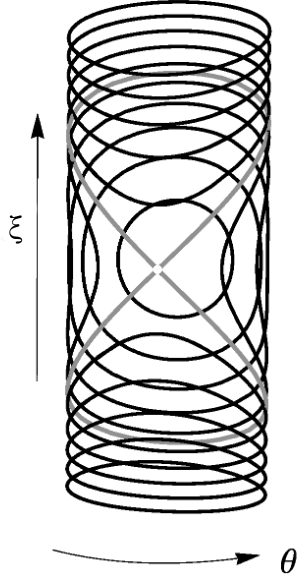
\includegraphics[width=.3\textwidth]{figures/pendulum_phase_space-cylinder.png}};
		\end{tikzpicture}
		\caption{The manifold $T^* S^1$, with compact fibers as solid black lines and open ones in grey.}
	\end{figure}
\end{example}

\begin{example}[Spherical pendulum]
	This time $M=T^*S^2$, we choose $\theta$ (longitude, $0 < \theta < 2\pi$) and $\phi$ (latitude, $0 < \phi < \pi$) as angle coordinates for $S^2$ and $\xi, \eta$ for the remaining ones. The Hamiltonian of the system is
	\begin{eqalign}
		h(\theta, \phi, \xi, \eta) = \frac12 \left(\eta^2 + \frac{\xi^2}{\sin^2\phi}\right) + \cos \phi
	\end{eqalign}
	whose differential is
	\begin{eqalign}
		dh = \eta d\eta + \frac{\xi}{\sin^2 \phi}d\xi - \left(\frac{\xi^2 \cos\phi}{\sin^3 \phi} + \sin\phi\right) d\phi
	\end{eqalign}
	which is singular iff $\eta=\xi=0$, $\phi=0,\pi$. Since $\dim S^2 = 2$, we need another integral of motion to apply Arnold--Liouville. Indeed, notice $h$ doesn't really depend on $\theta$! So we put $h_2=\xi$ ``$(=\dot \theta)$'' (check this commutes!).

	Let's check the points where $dh_1$ is not linearly indipendent from $dh_2$ (as with the singular points check for $dh$, this is in order to satisfy the hypothesis of Arnold--Liouville). As $dh_2 = d\xi$, this happens only when $dh_1$ has just the $d\xi$ term, i.e. the other two vanish:
	\begin{eqalign}
		\eta = 0, \quad \xi = \pm \sqrt{-\frac{\sin^4 \phi}{\cos \phi}}.
	\end{eqalign}
	Notice the condition on $\xi$ can be satisfied iff $\phi > \pi/2$ (since it is already less than $\pi$ by definition).

	On the singular points of $dh_1$, $X_{h_1} = X_{h_2} = 0$ (where the second equality is extended to the points outside the chosen chart by a simple continuity argument) while in the second set of points (where the differentials are not independent)
	\begin{eqalign}
		X_{h_1} &= \pm \frac1{\sqrt{-\cos\phi}} \partial_\theta\\
		X_{h_2} &= \partial_\theta
	\end{eqalign}
	The first case corresponds to the configurations where the pendulum is vertical, either upwards or downwards. The fact that the two Hamiltonian vector fields are zero tells us it has to stay still to maintain the balance. The second case represents circle orbits below the equator, those where gravity is balanced by centrifugal force.
\end{example}

\begin{exercise}
	Apply Arnold--Liouville Theorem to the ``updated'' phase space of the spherical pendulum, in particular describe the fibers of the Lagrangian fibration and the locus $M_C$ of the compact ones.
\end{exercise}

\begin{example}[Kepler's problem on the plane]
	Consider $M= T^*(\R^2 \setminus \{0\})$ with polar coordinates $r, \theta$ for the points and $p_r, p_\theta$ for covectors. The symplectic form on this manifold is
	\begin{eqalign}
		\omega = dr \wedge dp_r + d\theta \wedge dp_\theta
	\end{eqalign}
	along with Hamiltonian\footnote{We get this form from a suitable choice of description of the two-body system, from the reference frame of the center of mass.}
	\begin{eqalign}
		h = \frac{p^2_r}{2m} + \frac{p^2_\theta}{2mr^2} - \frac{k}{r}, \quad k,m > 0
	\end{eqalign}
	The two integrals of motion are then $h_1=h$ and $h_2 = p_\theta$.

	As before, we now study the linear independence of $dh_1, dh_2$. First of all, they are
	\begin{eqalign}
		dh_1 &= \frac{p_r}m dp_r + \frac{p_\theta}{mr^2}dp_\theta + \left( \frac{k}{r^2} - \frac{p_\theta^2}{mr^3} \right)dr\\
		dh_2 &= dp_\theta
	\end{eqalign}
	thus they're indipendent unless
	\begin{eqalign}
		p_r = 0, \quad r = \frac{p_\theta^2}{mk}
	\end{eqalign}
	which correspond to particular circular orbits.

	To find the fibers, choose an arbitrary point $c = (c_1, c_2) \in \R^2$. Hence the equations of a level set of $H = (h_1, h_2)$ are
	\begin{eqalign}
		\begin{dcases}
			c_1 = \frac{p_r^2}{2m} + V_{c_2}(r), \quad \text{where}\ V_{c_2}(r) = \frac{c_2^2}{2mr^2} - \frac{k}r\\
			c_2 = p_\theta
		\end{dcases}
	\end{eqalign}
	The term $V_{c_2}(r)$ is called the \emph{effective potential}. We then consider two cases.
	\begin{enumerate}
		\item $c_2 = 0$, yielding
		\begin{eqalign}
			c_1 = \frac{p_r^2}{2m} - \frac{k}r \implies r = \frac1k \frac1{\frac{p_r^2}{2m} - c_1}
		\end{eqalign}
		We observe that $r$ is free to be as large as we please, hence these fibers correspond to unbounded orbits of the system and, geometrically, to non-compact fibers.
		\item $c_2 \neq 0$, then inspecting the first equation we see that $c_1 < 0$ implies $V_{c_2}$ negative, thus when we draw its graph we notice this is only the case when $r < 0$. In this case, we get compact level sets. Clearly, the level set is empty whenever $c_1 < \min V_{c_2}(r)$.
	\end{enumerate}
	Therefore
	\begin{eqalign}
		H^{-1}(c_1, c_2) \begin{dcases}
			\text{is non-compact} = \R \times S^1 & \text{for $c_2 = 0$, $c_1 \geq 0$}\\
			= \T^2 & \text{when $c_2 \neq 0,\ - \frac{mk^2}{2c_2^2} < c_1 < 0$}\\
			= S^1 & \text{when $c_2 \neq 0,\ c_1 = -\frac{mk^2}{2c_2^2}$}\\
			= \varnothing & \text{when $c_2 \neq 0,\ c_1 < -\frac{mk^2}{2c_2^2}$}
		\end{dcases}
	\end{eqalign}
	Notice that the third case happens when $r= c_2^2/mk$, which we excluded previously for reasons of linear independence. Indeed, it represent a separatrix between compact and non-compact trajectories more or less like in the example of the pendulum. We can represent the fibration on the plane as such:

	\begin{figure}[H]
		\centering
		\begin{tikzpicture}
			\node (image) at (0,0) {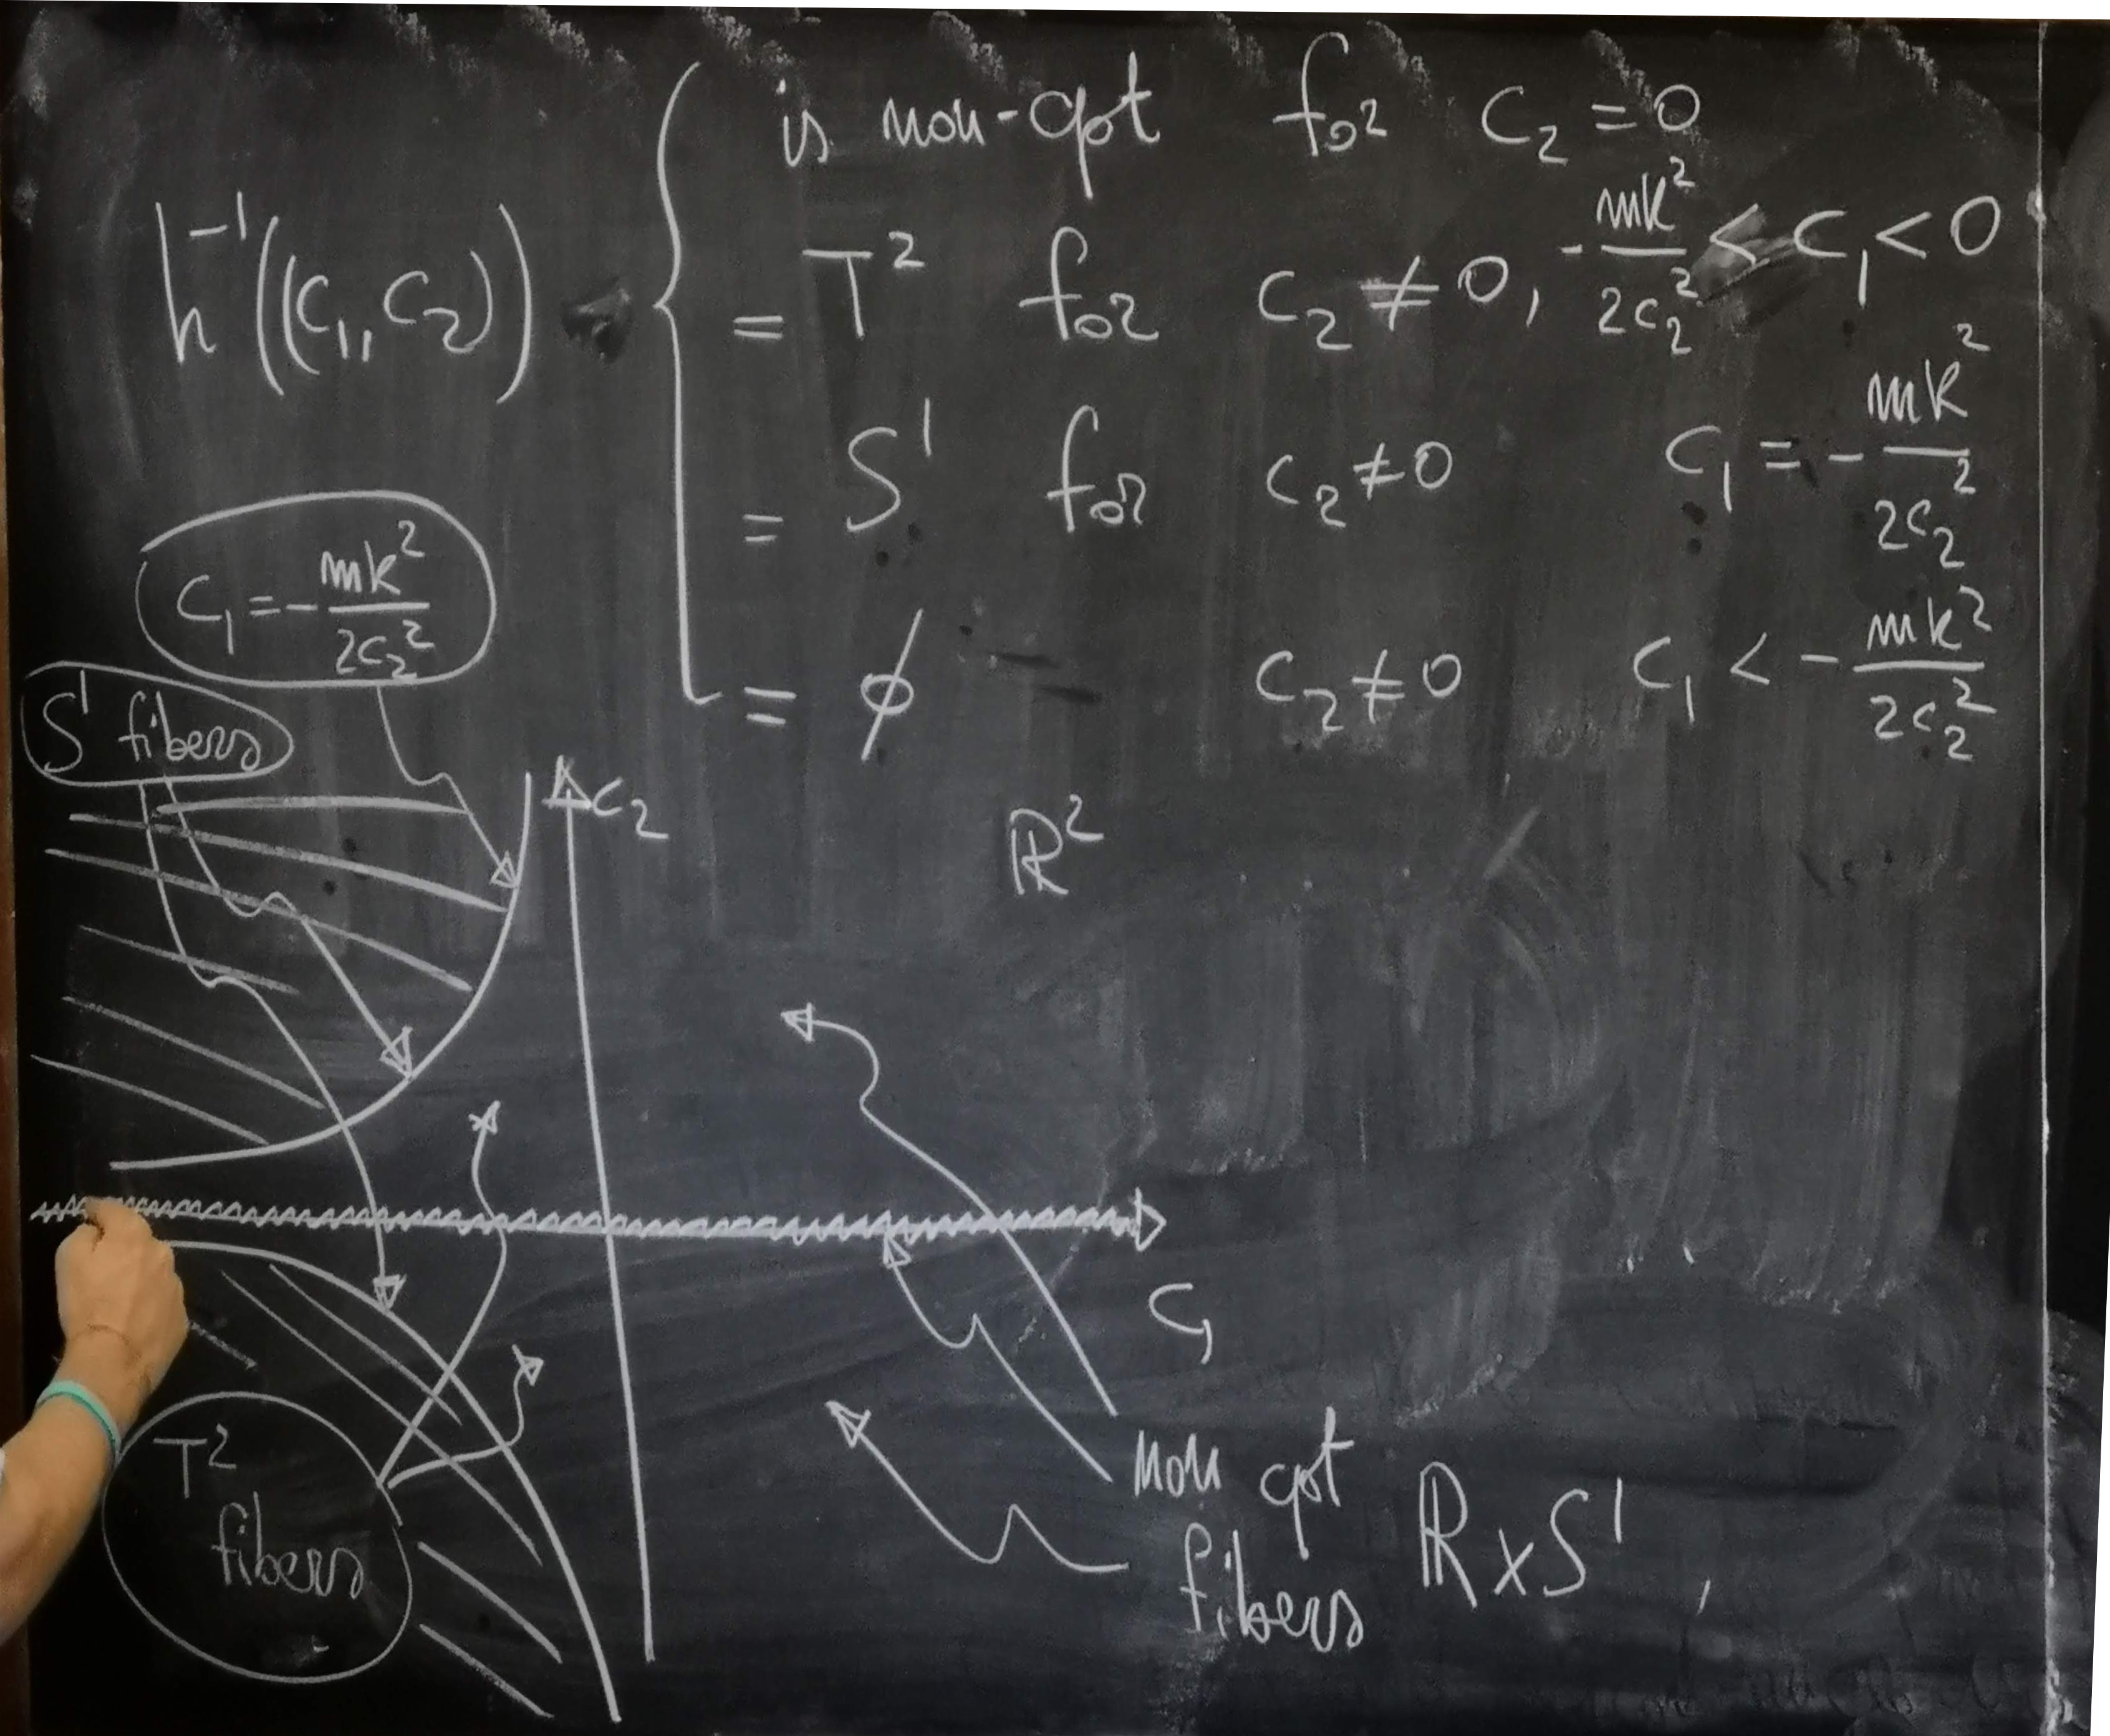
\includegraphics[width=.85\textwidth]{figures/mar28_fibers.jpg}};
		\end{tikzpicture}
	\end{figure}

	Thus the region of the plane giving compact fibers (i.e. tori) is
	\begin{eqalign}
		B = \left\{ (h, p_\theta) \in \R^2 \suchthat h < 0,\ 0 < |p_\theta| < k \sqrt{-m/2h} \right\}
	\end{eqalign}
	We can now move on to find the action-angle variables of the system: we start choosing $\gamma_1, \gamma_2$ basis for $H_1(H^{-1}(c_1, c_2))$. As the first one, we choose the circle in the $\theta$ direction parametrized by
	\begin{eqalign}
		\gamma_1 : S^1 &\longto H^{-1}(c_1, c_2)\\
		t &\overset{\theta}\longmapsto \begin{dcases}
			\theta = t\\
			r = \frac{-k + \sqrt{k^2 + \frac{c_1c_2^2}{m}}}{2c_1}\\
			p_r = 0\\
			p_\theta = c_2
		\end{dcases}
	\end{eqalign}
	The expression for $r$ is computed by imposing the circle to stay inside the fiber $H^{-1}(c_1, c_2)$, once we fixed $p_r=0$ (which is an arbitrary choice).

	The other loop $\gamma_2$, independent from $\gamma_1$, is naturally sought in the complementary part $(r,p_r)$
	of the fibers: as seen in Figure~\ref{fig:KeplerCompactFiber}, an $S^1$ is actually present (the disentanglement of the $r$-dynamics from the $\theta$-dynamics is due to the $\theta$-independence of $h$).

	\begin{figure}[H]
		\centering
		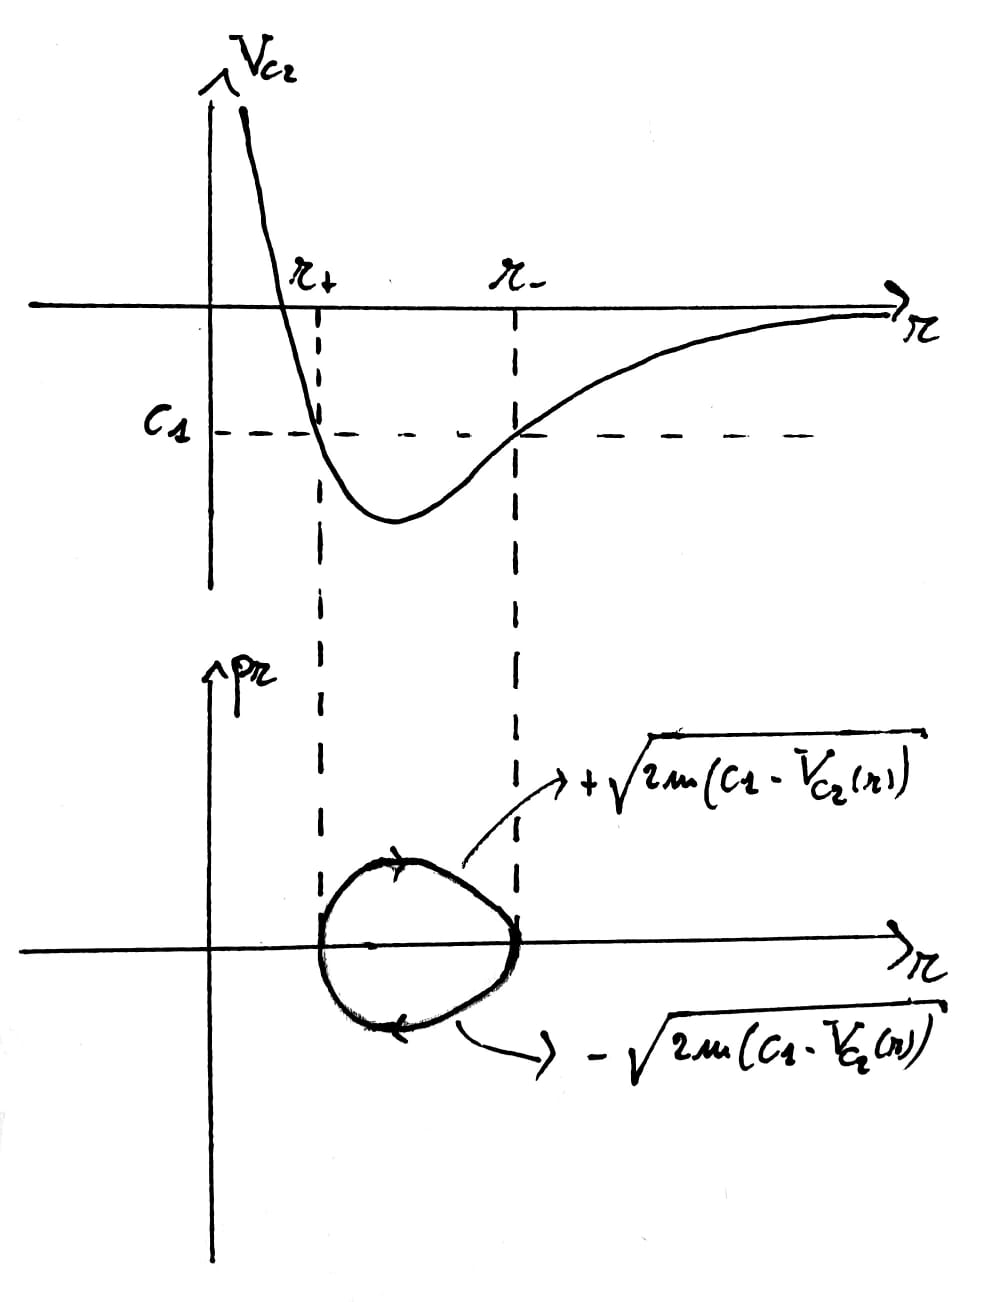
\includegraphics[width=.7\textwidth]{figures/KeplerCompactFiber.jpeg}
		\caption{}
		\label{fig:KeplerCompactFiber}
	\end{figure}
	\begin{figure}[H]
		\centering
		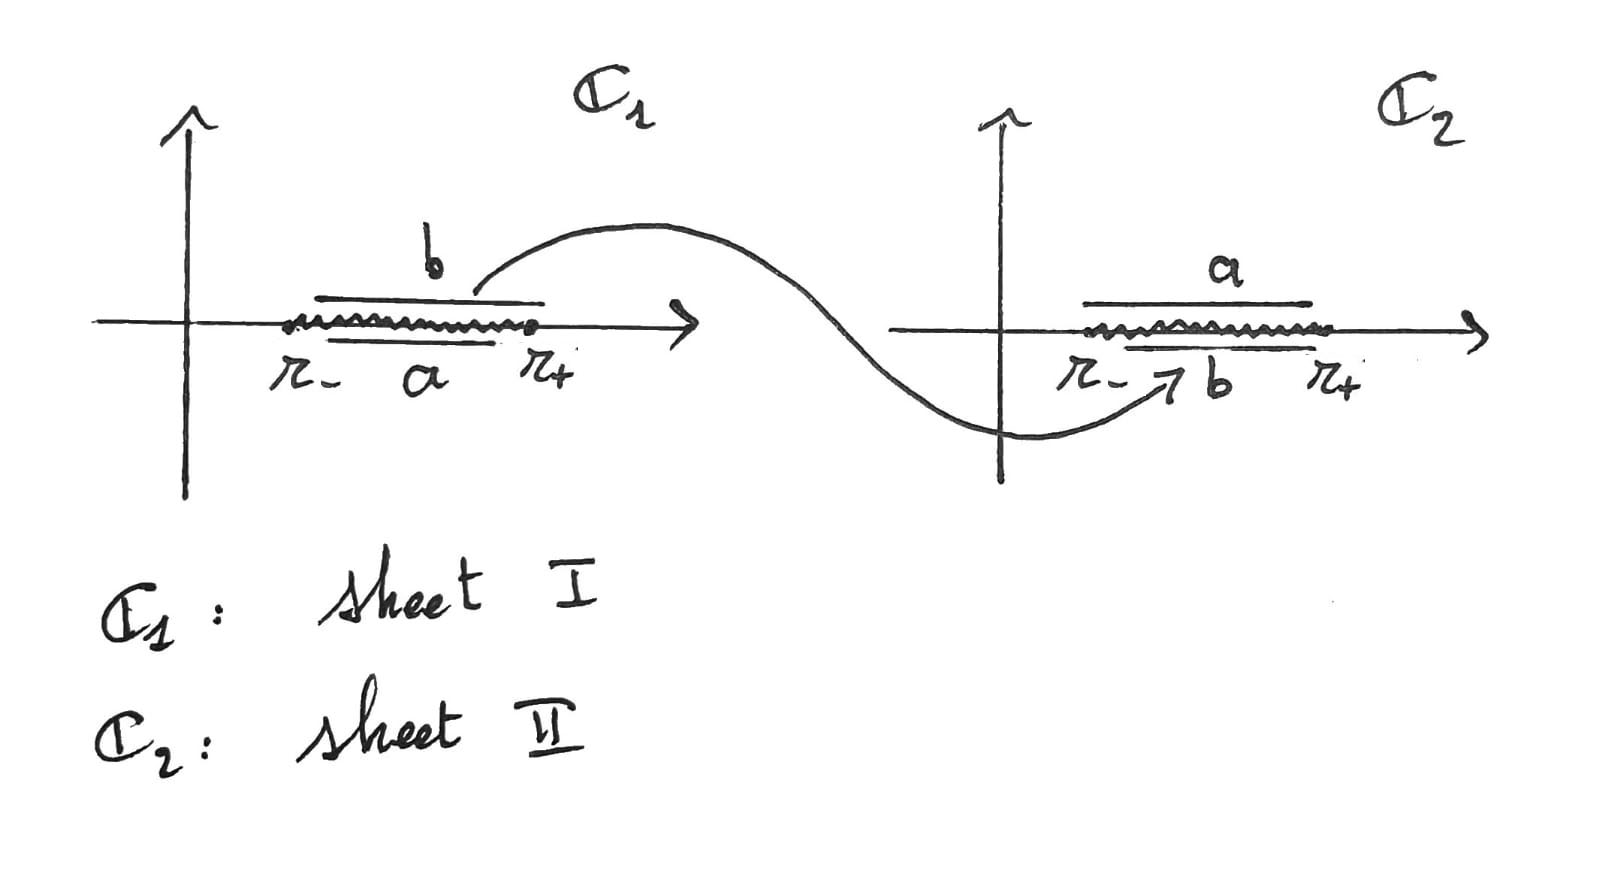
\includegraphics[width=.85\textwidth]{figures/MultivaluedFunctionDef.jpeg}
		\caption{}
		\label{fig:MultivaluedFunctionDef}
	\end{figure}

	Although harder to visualize, this should make clear why $\gamma_2$ can be chosen to be formed by two branches $\gamma^\pm_2$ stitched together at the ends:
	\begin{eqalign}
		\gamma_2^\pm : (r_+, r_-) &\longto H^{-1}(c_1, c_2)\\
		t &\longmapsto \begin{cases}
			\theta = 0 \comment{(arbitrary choice)} \\
			r= \pm t\\
			p_r = \pm \sqrt{2m \left(c_1 - V_{c_2}(\pm t) \right)}\\
			p_\theta = c_2
		\end{cases}
	\end{eqalign}
	The expression for $p_r$ is computed by imposing the circle to stay inside the fiber $H^{-1}(c_1, c_2)$, once we fixed $p_\theta=c_2$.
	The values $r_+$ and $r_-$ are given by the zeroes of the discriminant of $h_1=c_1$:
	\begin{eqalign}
	 r_\pm = \frac{-k \pm \sqrt{k^2 + \frac{c_1c_2^2}{m}}}{2c_1} \qquad (r_+<r_-).
	\end{eqalign}

	Put together, $\gamma_2$ goes go back and forth between $r_+$ and $r_-$ using the $p_r$ dimension.

	Then recall $\omega = d(-p_\theta d\theta - p_rdr)$, so, since $p_r=0$ on $\gamma_1$.
	\begin{eqalign}
		I_1(c_1, c_2) = - \int_{\gamma_1} (p_\theta d\theta + p_r dr) = -2\pi c_2
	\end{eqalign}
	As for computing $I_2$, $\gamma_2$ is obtained by spanning $r$ from $r_+$ to $r_-$ setting $p_r(r)=+g(r)$,
	and then spanning $r$ from $r_-$ to $r_+$ setting $p_r(r)=-g(r)$, where $g(r)=\sqrt{2m(c_1-V_{c_2}(r))}$, therefore
	\begin{eqalign}
		I_2(c_1, c_2) &= - \int_{\gamma_2} p_r dr \\
			      &= -\left(\int_{r_+}^{r_-} g(t) \,dt + \int_{r_-}^{r_+} (-g(t)) \,dt\right).
	\end{eqalign}
	To compute it, we use residues by interpreting the integral in the complex $t$ plane.

	In order to do that, we aim to rewrite $I_2$ as a circuit integral and then to deform the integration path using
	the properties of integrals of holomorphic functions.
	Let us start by defining the following function
	\begin{eqalign}
	 \pi_r(t)=\frac{\sqrt{-2mc_1}}{t}\sqrt{(t-r_-)(t-r_+)}.
	\end{eqalign}
	This is clearly a multivalued function on two sheets, I and II, with two branches.
	It displays only two ramification points in $r_\pm$, therefore we take the cut connecting them as shown in Figure~\ref{fig:MultivaluedFunctionDef}.
	Finally, it features a simple pole in zero, while being holomorphic elsewhere.

	Next, consider its restrictions to the real axis above and below the cut (respectively b and a sides): one easily gets
	\begin{eqalign}
	 \pi_r(t)_{|_b}&=ig(t)	\\
	 \pi_r(t)_{|_a}&=-ig(t)
	\end{eqalign}
	therefore one can consider the line integral
	\begin{equation}
	 I=\int_\gamma \pi_r(t)\,dt
	\end{equation}
	where $\gamma$ is the path shown in Figure~\ref{fig:IntPath}.

	\begin{figure}
	\centering
	\begin{minipage}{0.45\textwidth}
	\centering
	 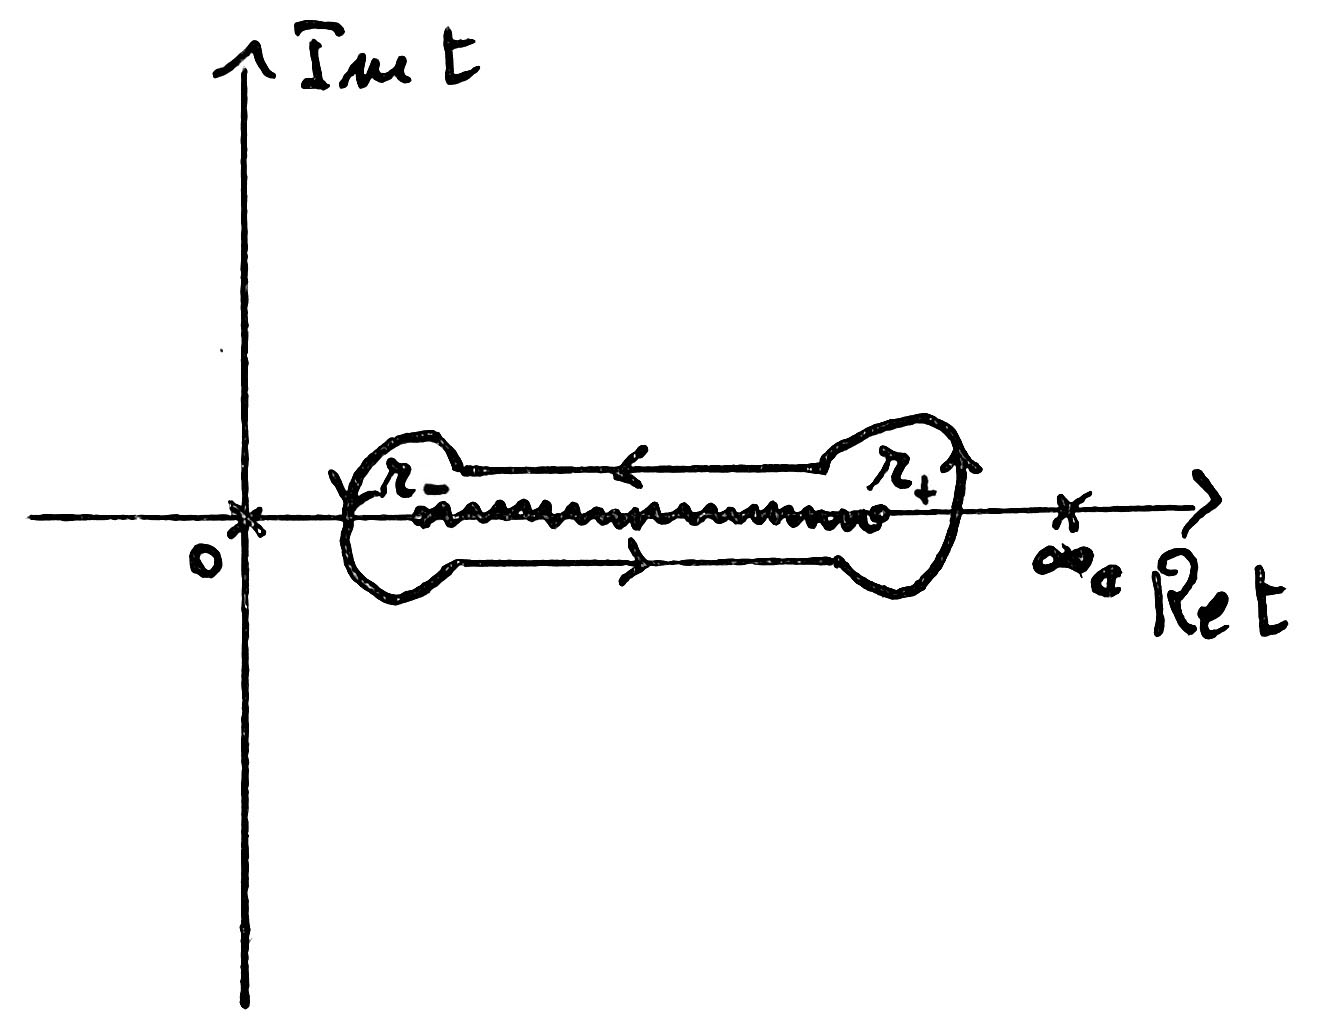
\includegraphics[width=\textwidth]{figures/IntPath.jpeg}
	 \captionof{figure}{}
	 \label{fig:IntPath}
	\end{minipage}
	\centering
	\begin{minipage}{0.5\textwidth}
	\centering
	 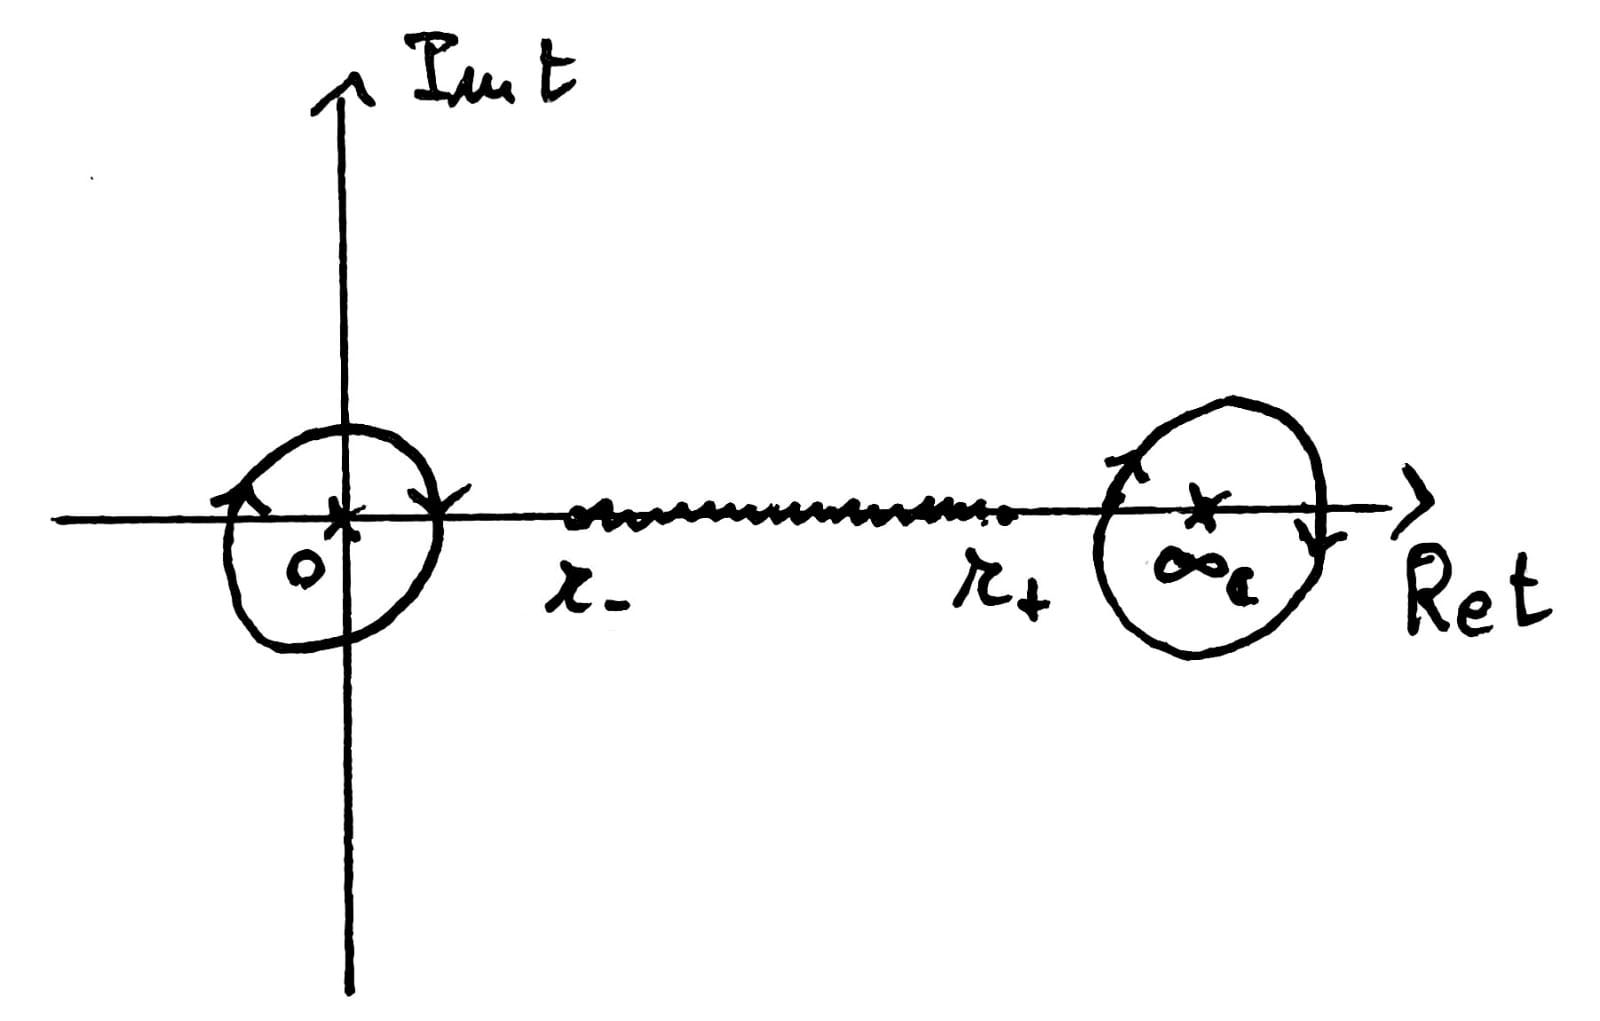
\includegraphics[width=\textwidth]{figures/ResidueIntPath.jpeg}
	 \captionof{figure}{}
	 \label{fig:ResidueIntPath}
	\end{minipage}
	\end{figure}

	One can continuously deform the integration path $\gamma$ without changing the result
	(since $\pi_r$ is holomorphic outside zero), so let us shrink $\gamma$ to the segment $[r_+,r_-]$, getting
	\begin{eqalign}
		I &=\int_{r_-}^{r_+}ig(x)\,dx+\int_{r_+}^{r_-}(-ig(x))\,dx\\
		  &=i\,I_2
	\end{eqalign}
	so that $I_2$ can actually be rewritten as
	\begin{equation}
		I_2(c_1,c_2)= -i\int_\gamma \pi_r(t)\,dt.
	\end{equation}

	Now we can use the residue theorem and trade $\gamma$ for the union of the circles $C_0$ and $C_\infty$ around
	the pole in zero and around $\infty_\C$ as integration path (see Figure~(\ref{fig:ResidueIntPath})).
	Keeping track of the inherited orientations of the circles, one gets
	\begin{eqalign}
	 I_2(c_1,c_2) &= \left(\int_{C_0} \pi_r(t) \,dt + \int_{C_\infty} \pi_r(t) \,dt\right)	\\
		      &= 2\pi i\left(-\underset{t=0}{\Res}(\pi_r(t))-\underset{t=\infty_\C}{\Res}(\pi_r(t))\right)
	\end{eqalign}

	Let us carry out the residue computation:
	\begin{enumerate}
	 \item \textbf{In $t=0$.} Let us expand $\pi_r$ in its Laurent series around $t=0$: one finds
			 \begin{equation}
			  \pi_r(t)=\frac{\sqrt{-2mc_1}}{t}\sqrt{r_+r_-}+\mathcal{O}(1),
			 \end{equation}
			 so that
			 \begin{eqalign}
			  \underset{t=0}{\Res}(\pi_r(t))&=\sqrt{-2mc_1r_+r_-}	\\
							&=c_2
			 \end{eqalign}
			 where we took $c_2>0$ and we used $r_+r_-=-\frac{c_2^2}{2mc_1}$.
	 \item \textbf{In $t=\infty_\C$.} Let us expand $\pi_r$ in its Laurent series around $t=\infty_\C$: one finds
			 \begin{equation}
			  \pi_r(t)=\sqrt{-2mc_1}-\frac{\sqrt{-2mc_1}(r_++r_-)}{2t}+\mathcal{O}(t^{-2}),
			 \end{equation}
			 therefore
			 \begin{eqalign}
			  \underset{t=\infty_\C}{\Res}(\pi_r(t))&=\frac{\sqrt{-2mc_1}}{2}(r_++r_-)	\\
							&=\frac{mk}{\sqrt{-2mc_1}}.
			 \end{eqalign}
	\end{enumerate}

	Finally, one gets
	\begin{eqalign}
	 I_2(c_1,c_2)&=-i\left[-2\pi i\Big(c_2+\frac{mk}{\sqrt{-2mc_1}}\Big)\right]	\\
		     &= -2\pi\left(c_2+\frac{mk}{\sqrt{-2mc_1}}\right).
	\end{eqalign}


	Reinserting back the functions for $c_1$ and $c_2$, one gets the following results:
	\begin{eqalign}
		I_1 &= -2\pi p_\theta\\
		I_2 &= -2\pi p_\theta - 2\pi \sqrt{\frac{mk^2}{-2 \left( \frac{p_r^2}{2m} + \frac{p_\theta^2}{2mr^2} - \frac{k}{r} \right)}}
	\end{eqalign}
	from which we can obtain the generalized momenta:
	\begin{eqalign}
		p_\theta &= -\frac1{2\pi} I_1\\
		p_r &= \sqrt{2m \left( -2\pi^2\frac{mk^2}{(I_2-I_1)^2} - \frac1{4\pi^2} \frac{I_1^2}{2mr^2} + \frac{k}{r} \right)}
	\end{eqalign}

	Call $\phi^\alpha$ the angle variables. Then
	\begin{eqalign}
		S(\theta, r, I_1, I_2) = \int_{(\phi_0, r_0)}^{(\theta, r)} (p_\theta d\theta + p_rdr)
	\end{eqalign}
	where the integration path is not relevant as long as it remains inside $H^{-1}(c_1, c_2)$. Then $\phi^\alpha = \partial S / \partial I_\alpha$, but \textbf{it's not possible to compute $S$ analytically}. However, we can still find the canonical transformation to get the action variables. We start by writing $h$ in terms of $I_1$ and $I_2$, an expression not depending on any other variable since $H$ is costant along the fibers. From the relative computation, we get
	\begin{eqalign}
		h=h(I_1, I_2) = 2\pi^2 \frac{mk^2}{(I_2 - I_1)^2}
	\end{eqalign}
	We know the equations of motion imply
	\begin{eqalign}
		\begin{dcases}
			\dot I_\alpha = 0 \comment{since it is an integral of motion}\\
			\dot\phi^\alpha = \pder{h}{I_\alpha} = \pm 4\pi^2 \frac{mk^2}{(I_2-I_1)^3}
		\end{dcases}
	\end{eqalign}
	Since $\phi^\alpha$ comes from the linear action on the torus, we can now get the angle coordinates:
	\begin{eqalign}
		\phi^\alpha = \dot\phi^\alpha t + \phi^\alpha_0
	\end{eqalign}

	The information we extracted from the system allows us, for example, to analyze the question of the periodicity of the motion. By computing the slope of the line described by the $\phi^\alpha$ on the toric fiber, we can answer positively that question:
	\begin{eqalign}
		\frac{\dot\phi^1}{\dot\phi^2} = -1 \in \Q
	\end{eqalign}
\end{example}

\begin{remark}
	The last part of the previous example shows an approach which works generally -- once we have $I_1, \ldots, I_n$, we can express $h$ in terms of them and then the angle variables as
	\begin{eqalign}
		\phi^\alpha = \pder{h(I_1, \ldots, I_n)}{I_\alpha} t + \phi^\alpha_0
	\end{eqalign}
\end{remark}

\end{document}